\def\year{2019}\relax
%File: formatting-instruction.tex
\documentclass[letterpaper]{article} %DO NOT CHANGE THIS
\usepackage{aaai19}  %Required
\usepackage{times}  %Required
\usepackage{helvet}  %Required
\usepackage{courier}  %Required
\usepackage{url}  %Required
\usepackage{graphicx}  %Required

%%%%%%%%%%%%%%%%%%%%%
\usepackage[bookmarks=true]{hyperref}
\usepackage{graphicx}
\usepackage[font=footnotesize]{subcaption}
\usepackage[font=footnotesize]{caption}
\usepackage{hyperref}
\usepackage{url}
\usepackage{amsmath,amssymb,amsfonts,amsfonts}
% \usepackage{algorithm}
% \usepackage[noend]{algorithmic}
\usepackage{xspace}
\usepackage{wrapfig}
\usepackage{color}
\usepackage{graphicx}

\usepackage{algorithm}
\usepackage{algorithmicx}
\usepackage[noend]{algpseudocode}
\usepackage{algpseudocode}
\usepackage{parskip}
\usepackage{amsthm}

\algrenewcommand\algorithmicindent{1.0em}%

\newcommand{\calX}{\ensuremath{\mathcal{X}}\xspace}
\newcommand{\calL}{\ensuremath{\mathcal{L}}\xspace}
\newcommand{\calS}{\ensuremath{\mathcal{S}}\xspace}
\newcommand{\calR}{\ensuremath{\mathcal{R}}\xspace}
\newcommand{\calD}{\ensuremath{\mathcal{D}}\xspace}

\newcommand{\sAttract}{\ensuremath{s^{\text{attractor}}_i}\xspace}
\newcommand{\sStart}{\ensuremath{s_{\text{start}}\xspace}}
\newcommand{\sGoal}{\ensuremath{s_{\text{goal}}\xspace}}
\newcommand{\sNom}{\ensuremath{s_{\text{nominal}}\xspace}}


\newtheorem{theorem}{Theorem}
\newtheorem{lemma}{Lemma}
\newtheorem{definition}{Definition}
\newtheorem{cor}{Corollary}
%%%%%%%%%%%%%%%%%%%

\frenchspacing  %Required
\setlength{\pdfpagewidth}{8.5in}  %Required
\setlength{\pdfpageheight}{11in}  %Required
%PDF Info Is Required:
  \pdfinfo{
/Title (Provable Infinite-Horizon Real-Time Planning for Repetitive Tasks)}
\setcounter{secnumdepth}{2}  
 \begin{document}
% The file aaai.sty is the style file for AAAI Press 
% proceedings, working notes, and technical reports.
%
\title{Provable Infinite-Horizon Real-Time Planning for Repetitive Tasks}
%\author{
%Fahad Islam,
%Oren Salzman {\normalfont and}
%Maxim Likhachev
%\\
%The Robotics Institute, Carnegie Mellon University\\
%%
%\{fi,osalzman\}@andrew.cmu.edu,
%maxim@cs.cmu.edu
%}
\maketitle

\begin{abstract}
In manufacturing, robots often have to perform highly-repetitive manipulation tasks in structured environments. 
In this work we are interested in the settings where the tasks are similar, yet not identical (e.g., due to uncertain orientation of objects) and motion planning needs to be extremely fast. 
Preprocessing-based approaches prove to be very beneficial in these settings---they analyze the configuration-space offline to generate some auxiliary information which can then be used in the query phase to speedup planning times. 
%
Typically, the tighter the requirement is on query times the larger the memory footprint will be. In particular, for high-dimensional spaces, providing real-time planning capabilities is impractical.
Moreover, as far as we are aware of, none of the general-purpose algorithms come with \emph{provable} guarantees on the real-time performance.
%
To this end, we propose a preprocessing-based method that provides provable bounds on the query time while incurring only a small amount of memory overhead in the query phase.
We evaluate our method on a 7-DOF robot arm and show a speedup of over tenfold in query time when compared to the \textsf{PRM} algorithm, while guaranteeing a maximum query time of less than 4 milliseconds.
\end{abstract}

\section{Introduction}
%1. What is the problem?
We consider the problem of planning robot motions for highly-repetitive tasks while ensuring bounds on the planning times.
%2. Why is it relevant?
As a running example, consider the problem of a robot picking up objects from a high-speed conveyor belt and placing them into bins (see Fig.~\ref{fig:PR2}).
While the environment does not change, the start and goal in each task are similar, yet not identical to the start and goal in previous tasks.
Differences in the exact start and goal positions may be due to uncertainty in the environment as objects may be placed on different parts of the conveyor belt or in different orientations.
Fast planning times immediately correspond to faster unloading capabilities. 
Moreover, if the planner cannot \emph{guarantee} to pick items from the conveyor in a timely manner, the system is required to account for missed items by e.g., additional conveyor belts that will redirect items back to the robot---a costly backup in terms of both time and space.

%3. Why is it hard?
Clearly, every time a task is presented to the robot, it can compute a desired path.
However, this may incur large online planning times that may be unacceptable in many settings.
%
Alternatively, we could attempt to precompute for each start and goal pair a robot path.
However, as the set of possible start and goal locations may be large, caching pre-computed paths for all these queries in advance is unmanageable in high-dimensional configuration spaces.
Thus, we need to balance memory constraints while providing provable real-time query times.

\begin{figure}[tb]
  \centering
    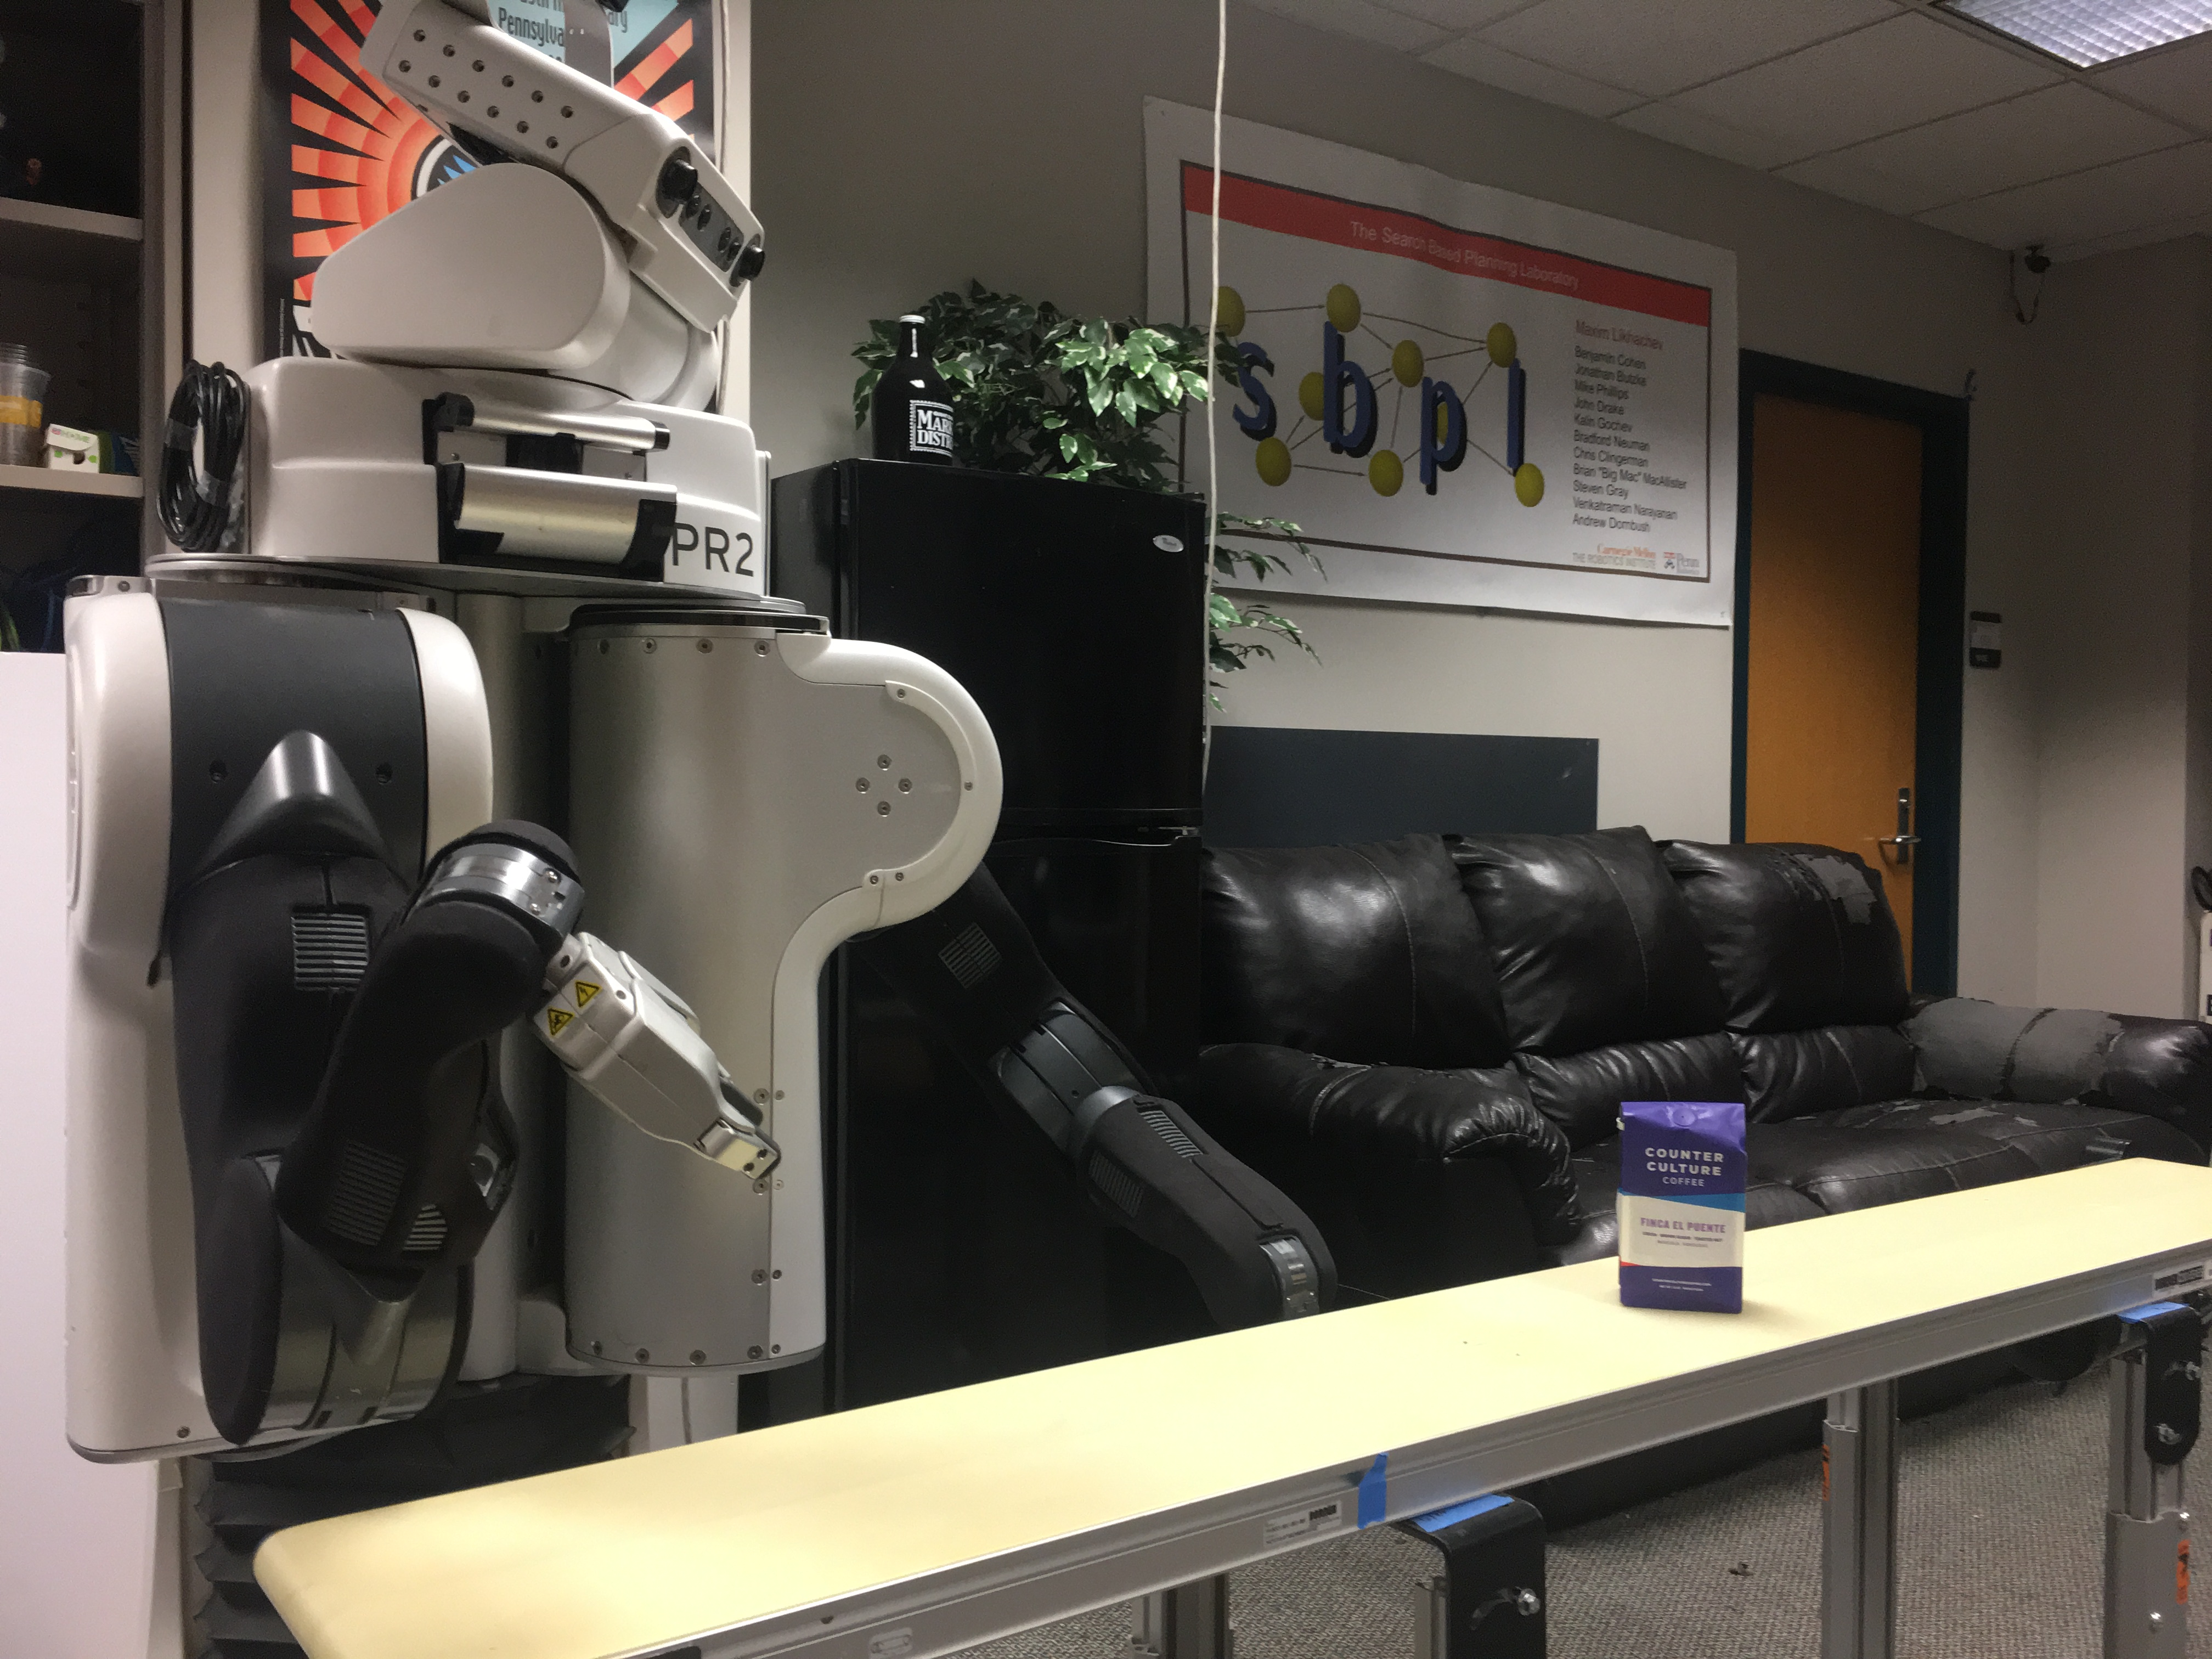
\includegraphics[width=0.35\textwidth]{PR2.jpg}
    % \vspace{-2mm}
  \caption{
  Motivating scenario---a robot (PR2) picking up objects from a conveyor belt.
}
    \label{fig:PR2}
% \vspace{-6mm}
\end{figure}

%4. What have others done?
As we detail in Sec.~\ref{sec:rel}, there has been intensive work 
for fast online planning~\cite{LA18} and 
for learning from experience in known environments~\cite{PCCL12,PDCL13,BAG12,CSMOC15}.
Similarly, compressing precomputed data structures in the context of motion-planning is a well-studied problem with efficient algorithms~\cite{SSAH14,DB14}.
%5. What's missing?
However, to the extent of our knowledge, there is no approach that can \emph{provably guarantee} that a solution will be found to \emph{any} query with bounds on planning time and using a low memory footprint.

%6. What is our ONE key insight?
Our key insight is that given any state $s$, we can efficiently compute a set of states for which a greedy search towards~$s$ is collision free.
Importantly, the runtime-complexity of such a greedy search is bounded and there is no need to perform computationally-complex collision-detection operations. 
This insight allows us to generate in an offline phase a small set of so-called ``attractor vertices'' together with a path between each attractor state and the goal.
In the query phase, a path is generated by performing a greedy search to an attractor state followed by the precomputed path to the goal.
We describe our approach in Sec.~\ref{sec:alg} and analyze it In Sec.~\ref{sec:analysis}

%7. How do we compare against the state of the art?
We evaluate our approach in Sec.~\ref{sec:eval} in simulation on the PR2 robot\footnote{http://www.willowgarage.com/pages/pr2/overview} (see Fig.~\ref{fig:PR2}).
We demonstrate a speedup of over tenfold in query time when compared to the \textsf{PRM} algorithm with a little memory footprint if 0.2 Mbs and while guaranteeing a maximal query time of less than 4 milliseconds.

%8. What are our contributions?
%9. What are our limitations?

\section{Related work}
\label{sec:rel}
A straightforward approach to efficiently preprocess a known environment is using the \textsf{PRM} algorithm~\cite{kavraki1996probabilistic} which generates a \emph{roadmap}.
Once a a dense roadmap has been pre-computed, any query can be efficiently answered online by connecting the source and goal to the roadmap. 
Query times can be significantly sped up by further preprocessing the roadmaps using landmarks~\cite{paden2017landmark}.
Unfortunately, there is no guarantee that a query can be connected to the roadmap as \textsf{PRM} only provides \emph{asymptotic} guarantees~\cite{KKL98}.
Furthermore, this connecting phase requires running a collision-detection algorithm which is typically considered the computational bottleneck in many motion-planning algorithms~\cite{L06}.

Recently, Lehner and  Albu{-}Sch{\"{a}}ffer~\cite{LA18} suggest the repetition roadmap to extend the \textsf{PRM} for the case of multiple highly-similar scenarios.
While their approach exhibits significant speedup in computation time, it still suffers from the previously-mentioned shortcomings.

A complementary approach to aggressively preprocess a given scenario is by minimizing collision-detection time.
However this requires designing robot-specific
circuitry~\cite{MFQSK16}
or limiting the approach to standard manipulators~\cite{YMILV18}.

An alternative approach to address our problem is to precompute a set of complete paths into a library and given a query, attempt to match complete paths
from the library to the new query~\cite{berenson2012robot,jetchev2013fast}.
Using paths from previous search episodes (also known as using experience) has also been an active line of work~\cite{PCCL12,PDCL13,BAG12,CSMOC15}.
Some of these methods have been integrated with sparse motion-planning roadmaps (see e.g.,~\cite{SSAH14,DB14}) to reduce the memory footprint of the algorithm.
Unfortunately, non of the mentioned algorithms provide any of the guarantees required by our applications.

Our work bares resemblance to previous work on 
subgoal graphs~\cite{UK17,UK18} and to real-time planning~\cite{KL06,KS09,K90}.
However, in the former, the entire configuration space is preprocessed in order to efficiently answer queries between \emph{any} pair of states which deems it applicable only to low-dimensional spaces.
{\color{blue} Also their $connect$ step is expensive as it requires a Dijkstra's like search to connect to the subgoal graph.} Similarly, in the latter, to provide guarantees on planning time the search only looks at a finite horizon and interleaves planning and execution.


Finally, our notion of attractor states is similar to control-based methods that  ensure safe operation over local regions of the free configuration space~\cite{CRC03,CCR06}.
These regions are then used within a high-level motion planner to compute collision-free paths.

% 
%\begin{itemize}
%	\item Sampling-based roadmaps
%		\begin{itemize}
%			\item PRM
%			\item Improve query using landmarks~\cite{paden2017landmark}.
%			\item Repetition roadmap~\cite{LA18} 
%		\end{itemize}
%	\item Minimize CD time
%		\begin{itemize}
%			\item robot-specific
%circuitry~\cite{MFQSK16}
%			\item limiting the approach to standard manipulators~\cite{YMILV18}.
%		\end{itemize}
%	\item Subgoal graphs
%	\item Experience 
%		\begin{itemize}
%			\item E-graphs~\cite{PCCL12,PDCL13}
%			\item THUNDER~\cite{CSMOC15}
%		\end{itemize}
%	\item Control-based funneling
%		\begin{itemize}
%			\item ensure safe operation over local regions of the free configuration space;~\cite{CRC03,CCR06}
%			\item  a method of composing
%simple control policies, applicable over a limited region in a dynamical system’s free space, such that the resulting composition completely solves the navigation and contro~\cite{CRC03}
%		\end{itemize}
%%	\item Compressing roadmaps~\cite{SSAH14,DB14}
%\end{itemize}



\section{Algorithm Framework}
\label{sec:alg}
In this section we describe our algorithmic framework. We start (Sec.~\ref{sec:pdef}) by formally defining our problem and continue (Sec.~\ref{sec:key}) by describing the key idea that enables our approach.
We then proceed (Sec.~\ref{subsec:alg}) to detail our algorithm and conclude (Sec.~\ref{subsec:impl})

\subsection{Problem formulation and assumptions}
\label{sec:pdef}
Let $\calX$ be the configuration space of a robot operating in a static environment.
We are given in advance a start configuration~$\sStart \in \calX$ and some goal region~$G \subset \calX$.
In the query phase we are given multiple queries $(\sStart, s_{\text{goal}})$ where $s_{\rm goal} \in G$ and for each query, we need to compute a collision-free path connecting $\sStart$ to $s_{\text{goal}}$.

We discretize $\calX$ into a state lattice $\calS$ such that any state~$s \in \calS$ is connected to a set of successors via a mapping Succs: $\calS \rightarrow 2^\calS$
and set $G_\calS := \calS \cap G$ to be the states that reside in the goal region.
We make the following assumptions:

\begin{enumerate}
  \item[\textbf{A1}] $G_\calS$ is a relatively small subset of $S$. Namely, it is feasible to exhaustively iterate over all states in $G_\calS$.
However, storing a path from $\sStart$ to each state in $G_\calS$ is infeasible.
  
  \item[\textbf{A2}] The planner has access to a heuristic function $h: \calS \times \calS \rightarrow \mathbb{R}$ which can estimate the distance between any two states in $G_\calS$. Moreover the heuristic function should be $\textit{weakly-monotonic}$, meaning that $\forall s_1, s_2  \in G_\calS$ where $s_1 \neq s_2 $, it holds that,

  \begin{center}
    $h(s_1, s_2) \geq \min\limits_{s_1' \in \text{Succs}(s_1)} h(s_1', s_2)$. 
  \end{center}
  Namely, for any distinct pair of states ($s_1, s_2$) in $G_\calS$, at least one of $s_1$'s successors (also belonging to $G_\calS$) must have a heuristic value less than or equal to its heuristic value.
	Note that this assumption does not imply  that~$G$ is entirely collision free.

  \item[\textbf{A3}] The planner has access to a tie breaking rule that can be used to define a total order \footnote{A total order is a binary relation on some set which is antisymmetric, transitive, and a connex relation.} over all states with the same heuristic value to a given state.
  \end{enumerate}

These assumptions allow us to establish strong theoretical properties regarding the efficiency of our planner. Namely, that
within a known bounded time, we can compute a collision-free path from $\sStart$ to any state in $G_\calS$. 
%Proofs are omitted due to lack of space. 

\subsection{Key idea}
\label{sec:key}
{\color{blue} Add a figure that demonstrates the complete approach.}

Our algorithm relies heavily on the notion of a greedy search.  Thus, before we provide an overview of our algorithm, we formally define the notions of greedy successor and greedy search.

\vspace{2mm}
\begin{definition}
	Let $s$ be some state and $h(\cdot)$ be some heuristic function.
	A state $s' \in \text{Succ}(s)$ is said to be a \emph{greedy} successor of $s$ according to $h$ if it has the minimal $h$-value among all of $s$'s successors.
\end{definition}
Note that 
if $h$ is weakly monotone 
(Assumption~\textbf{A2}) 
and we have some tie-breaking rule
(Assumption~\textbf{A3}), then the greedy successor of a state is unique.  
In the rest of the text, when we use the term greedy successor, we assume that it is unique.

\vspace{2mm}
\begin{definition}
	Given a heuristic function $h(\cdot)$,
	an algorithm is said to be a \emph{greedy search} if for every state it returns its greedy succesor.
\end{definition}

Our key insight is to precompute in an offline phase regions where a greedy search to a certain state is guaranteed to be collision free and use these regions in the query phase.
Specifically,
%Our planner comprises of a preprocessing and a query phase. 
in the preprocessing phase, $G_\calS$ is decomposed into two finite  sets of (possibly overlapping) subregions $\calR$ and~$\hat{\calR}$.
Subregions in $\hat{\calR}$ only contain states that are in collision.
Each subregion $R_i \in \calR$ is a hyper-ball defined using a center which we refer to as the ``attractor state''~
\sAttract and a radius $r_i$.
% centered around what we call the $attractor$ states $s_{attractor_i}$ and radii $r_i$, where $i$ = 1 to $n$. 
These regions are constructed in such a way that the following two properties hold
\begin{enumerate}
  \item[\textbf{P1}] For any goal state $s_{\text{goal}} \in R_i \cap G_\calS$, a greedy search with respect to $h(s, \sAttract)$ over $\calS$ starting at $\sGoal$ will result in a collision-free path to \sAttract.
  \item[\textbf{P2}] The union of all the subregions completely cover $G_\calS$. 
		  Namely, $\forall s \in G_\calS, \exists R \in \calR \cup \hat{\calR} \ s.t. \ s \in R$.
  		%In other words, any query state $\sGoal \in G$ will fall in atleast one of the subregions.
\end{enumerate}

In the preprocessing stage, we precompute a library of collision-free paths $\calL$ which includes one path from $\sStart$ to each attractor state. 
In the query phase, given a query~\sGoal, we 
(i)~identify a region $R_i$ such $\sGoal \in R_i$ (using the precomputed radii~$r_i$),
(ii)~run a greedy search towards~\sAttract by greedily choosing at every point the successor that minimizes~$h$ and
(iii)~append this path with the precomputed path in $\calL$ to $\sStart$ to obtain the complete plan.

\subsection {Algorithm}
\label{subsec:alg}
\subsubsection{Preprocessing Phase}
The preprocessing phase of our algorithm, detailed in Alg.~\ref{alg:1}, takes as input the start state~$\sStart$ and the goal region~$G_\calS$ and outputs a set of subregions~$\calR$ and the corresponding library of paths~$\calL$ from each \sAttract to~\sStart. 

The algorithm covers~$G_\calS$ by iteratively finding a state $s$ not covered\footnote{Here, a state $s$ is said to be covered if there exists some region $R \in \calR$ such that $s \in R$.} by any region and computing a new region centered at $s$.
To ensure that $G_\calS$ is complete covered (Property~\textbf{P2}) we maintain a set~$V$ of valid (collision free) and a set $I$ of invalid (in collision) states called \emph{frontier states} (lines~\ref{alg:1:v} and~\ref{alg:1:i}, respectively).
We start by initializing~$V$ with some random state in $G_\calS$ and iterate until both~$V$ and~$I$ are empty, which will ensure that $G_\calS$ is indeed covered.

At every iteration, we pop a state from $V$ (line~\ref{alg:1:pop}), and if there is no region covering it, we add it as a new attractor state and compute a path $\pi_i$ to $\sStart$ (line~\ref{alg:1:path}).
We then compute the corresponding region (line~\ref{alg:1:cr} and Alg.~\ref{alg:2}).

As we will see shortly, computing a region corresponds to a Dijkstra-like search centered at the attractor state.
The search terminates with the region's radius $r_i$ and a list of frontier states that comprise of the region's boundary.
The valid and invalid states are then added to $V$ and $I$, respectively (lines~\ref{alg:1:insert_v} and~\ref{alg:1:insert_i}).


Once $V$ gets empty the algorithm starts to search for states which are valid and yet uncovered by growing regions around the states popped from~$I$ (lines~\ref{alg:1:iv_loop}-\ref{alg:1:iv_region}). If a valid and uncovered state is found, it is added to $V$ and the algorithm goes back to computing subregions (lines~\ref{alg:1:x_states}-\ref{alg:1:break}), otherwise if $I$ also gets empty, the algorithm terminates and it is guaranteed that each valid state contained in $G_\calS$ is covered under at least one subregion.

\begin{algorithm}[t]
\footnotesize
\hspace*{\algorithmicindent} \textbf{Inputs:} $G_\calS$, $\sStart$
\Comment{goal region and start state} 

\hspace*{\algorithmicindent} \textbf{Outputs:} 
$\calR, \calL$
%$R_i = (\sAttract, r_i)$, $\pi_i$,
\Comment{subregions and corresponding paths to $\sStart$}

%\hspace*{\algorithmicindent}
% \textbf{Parameters:} $r_{\text{max}}$   \Comment{maximum radius of a region}
\caption{Goal Region Preprocessing}\label{alg:1}


\begin{algorithmic}[1]
\Procedure{PreprocessRegion}{$G_\calS$}
%\Procedure{PreprocessRegion}{$G, r_{\text{max}}$}
  \State $s \leftarrow$\textsc{ SampleValidState}($G_\calS$)
  \State $V \leftarrow \{ s \}$   \Comment{valid frontier states initialized to a random state} \label{alg:1:v}
  \State $I$ = $\emptyset$   \Comment{invalid frontier states} \label{alg:1:i}
  \State $ i \leftarrow 0$
  		 \hspace{2mm} 
  		 $\calL = \emptyset$
  		 \hspace{2mm} 
  		 $\calR = \emptyset$
  		 \hspace{2mm} 
  		 $\hat{\calR} = \emptyset$
  		 
  \vspace{2mm}
    \While {$V$ and $I$ are not empty}
        \While {$V$ is not empty}
          \State $s \leftarrow V.\text{pop}()$ \label{alg:1:pop}
            \If {$\nexists R \in \calR$  s.t. $s \in R$ }  \label{alg:1:discard}
            \Comment{$s$ is not covered}
				\State $\sAttract \leftarrow s$               
				\label{alg:1:attract} 
                \State $\pi_i$ = \textsc{PlanPath}($\sAttract , \sStart$);	\label{alg:1:pp}
                \hspace{2mm }
                $\calL \leftarrow \calL \cup \{ \pi_i \}$  \label{alg:1:path}
                \State $(\text{OPEN}, r_i) \leftarrow$ \textsc{ComputeReachability}($\sAttract$) \label{alg:1:cr}
%                \State $(\text{OPEN}, r_i) \leftarrow$ \textsc{ComputeReachability}($\sAttract, r_{\text{max}}$) \label{alg:1:cr}
                \State insert Valid(OPEN) in $V$  \label{alg:1:insert_v}
                \State insert Invalid(OPEN) in $I$   \label{alg:1:insert_i}
                \State $R_i$ $\leftarrow$ $(\sAttract, r_i)$; 
                \hspace{2mm} $ i \leftarrow i+1$				\hspace{2mm }
                $\calR \leftarrow \calR \cup \{ R_i \}$
                            \EndIf
        \EndWhile

\vspace{2mm}        
        
        \While {$I$ is not empty} \label{alg:1:iv_loop}
            \State $s$ $\leftarrow$ $I.pop()$
			\If {$\nexists R \in \calR \cup \hat{\calR}$ s.t. $s \in R$ }      \Comment{$s$ is not covered}
\State $(X, r)$ $\leftarrow$ \textsc{SearchValidUncoveredStates}($s$)
%                \State $(X, r)$ $\leftarrow$ \textsc{SearchValidUncoveredStates}($s, r_{\text{max}}$)
                \State $\hat{R}$ $\leftarrow$ $(s,r)$;
				\hspace{2mm}
				$\hat{\calR} \leftarrow \hat{\calR} \cup \{ \hat{R} \}$ \Comment{invalid region}  \label{alg:1:iv_region}
                \If {$X$ is not empty}  \Comment{no valid state found}  \label{alg:1:x_states}
                    \State insert $X$ in $V$
                    \State \textbf{break} \label{alg:1:break}
                \EndIf
            \EndIf
        \EndWhile
    \EndWhile

  \vspace{2mm}

  \State \Return $\calR, \calL$
\EndProcedure
\end{algorithmic}
\end{algorithm}

\begin{figure}[tb]
  \centering
  	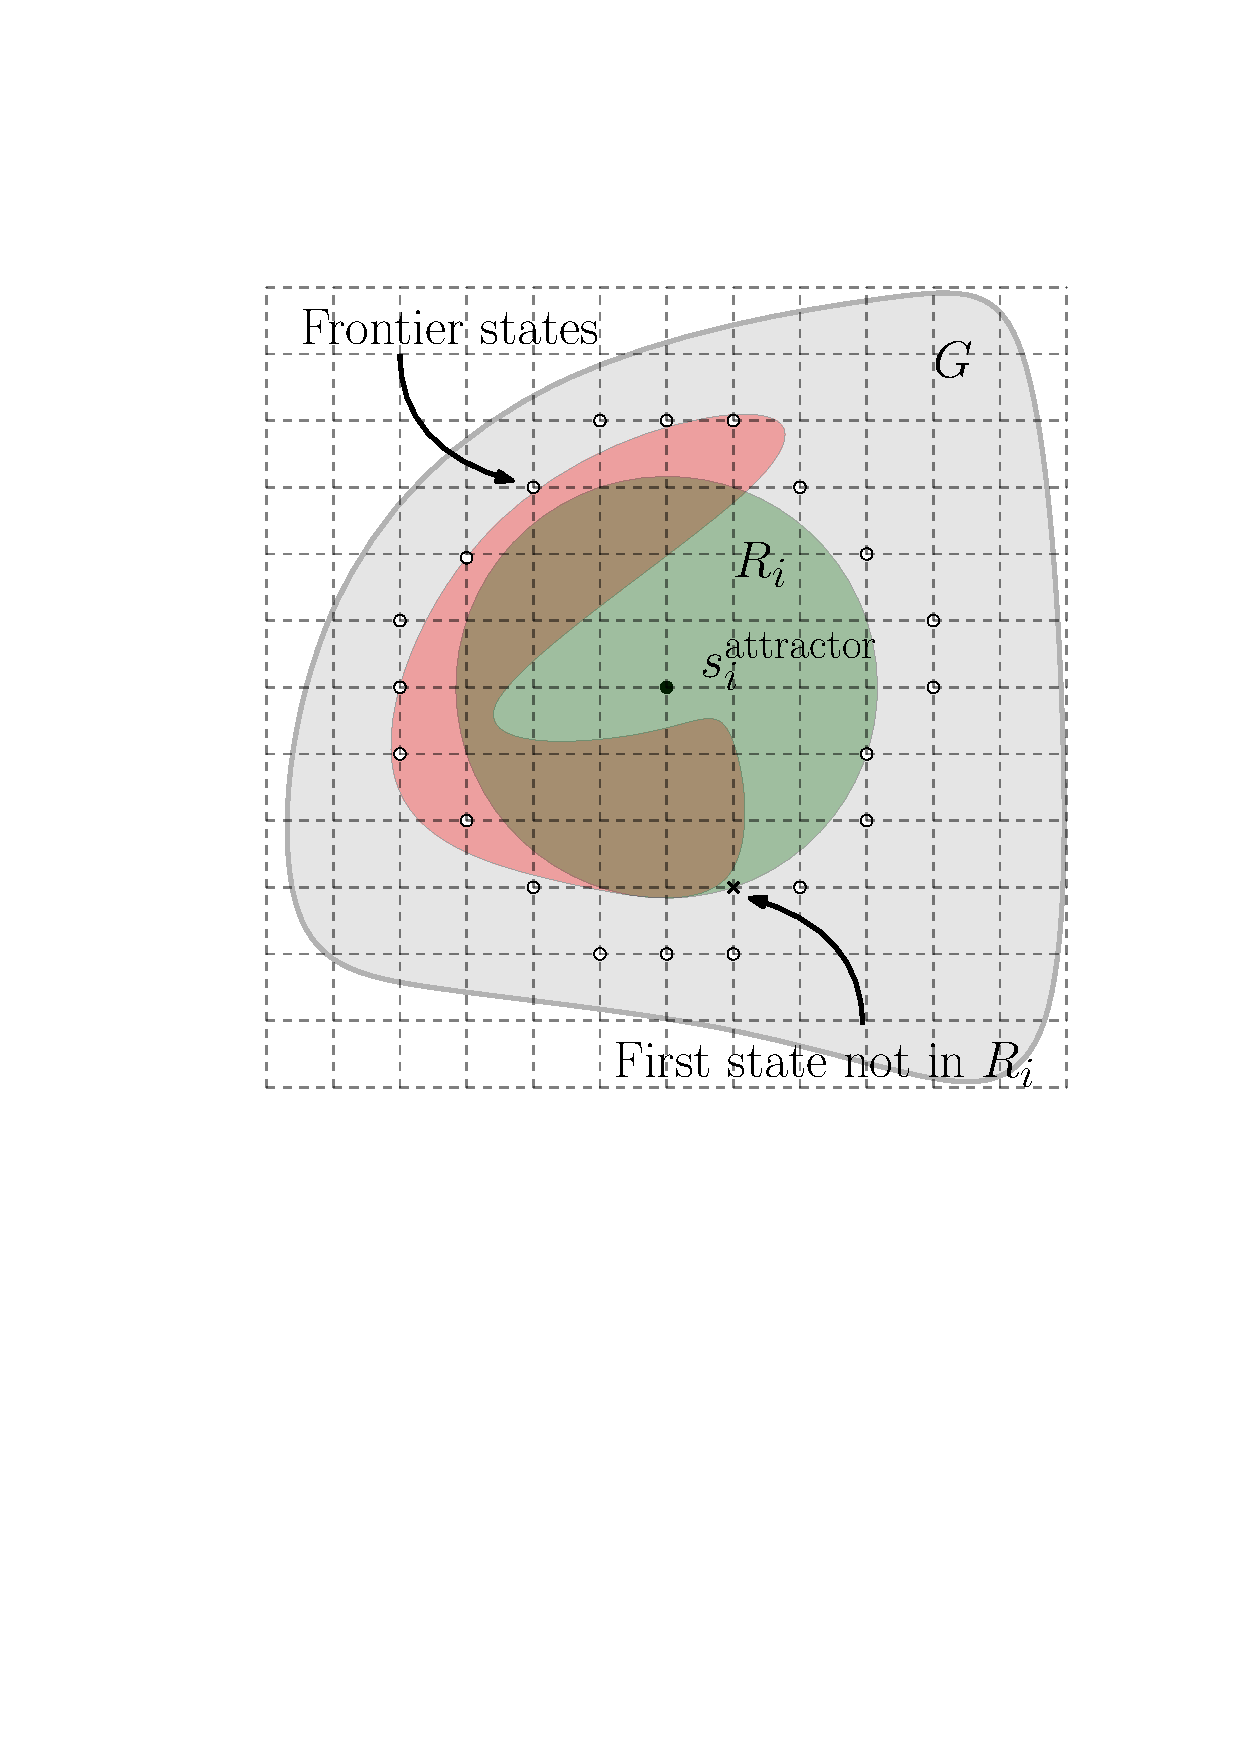
\includegraphics[width=0.20\textwidth]{Alg2.pdf}
  	% \vspace{-2mm}
  \caption{
  Visualization of Alg~\ref{alg:2}. Subregion $R_i$ (green) grown from $\sAttract$ in a goal region~$G_\calS$ (grey) containing an obstacle (red).
  Frontier states  and first state not in $R_i$ are depicted by circles and a cross, respectively.
}
   	\label{fig:alg2}
% \vspace{-6mm}
\end{figure}

\subsubsection{Reachability Search}
The core of our planner lies in the way we compute the subregions (Alg.~\ref{alg:2} and Fig.~\ref{fig:alg2}) which we call a ``Reachability Search''. The algorithm maintains a set of \emph{reachable} states $S_{\text{reachable}}$ for which property \textbf{P1} holds.
As we will see this will ensure that in the query phase, we can run a greedy search from any reachable state $s \in S_{\text{reachable}}$ and it will terminate in the attractor state. 
%
The following definition formally captures the notion of a reachible state.

\vspace{2mm}
\begin{definition}
	Given some attractor state \sAttract, a state $s$ is said to be reachable with respect to \sAttract if either
	(i)~$s = \sAttract$ or
	(ii)~the greedy successor of $s$ is reachable respect to \sAttract.
\end{definition}

%Namely, the greedy successor $s'$ of every reachable state $s \in S_{\text{reachable}}$ is also a reachable state, except for the attractor state \sAttract. 
%This will ensure that in the query phase, we can run a greedy search from any reachable state $s \in S_{\text{reachable}}$ and it will terminate in the attractor state. 

The algorithm computes a subregion that covers the maximum number of reachable states that can fit into a hyper-ball defined by $h(s,\sAttract)$. 
The search maintains a priority queue OPEN ordered according to $h(s,\sAttract)$. Initially, the predecessors of $\sAttract$ are inserted in the OPEN (line~\ref{alg:2:OPEN}). For each expanded predecessor, if its valid greedy successor is in $S_{\text{reachable}}$, then the predecessor is also labeled as reachable (lines~\ref{alg:2:crit} and~\ref{alg:2:set}). 
%As the priority used for OPEN is the heuristic function, the radius of this hyper-ball keeps on increasing (line~\ref{alg:2:rad}). 


The algorithm terminates when the search pops a state which is valid but does not have a greedy successor state in $S_{\text{reachable}}$ (line~\ref{alg:2:terminate}). Intuitively, this corresponds to the condition when the reachability search exists an obstacle (see Fig.~\ref{fig:alg2}). At termination, all the states within the boundary of radius $r_i$ (excluding the boundary) are reachable.


\begin{algorithm}[t]
\footnotesize
\caption{Reachability Search}\label{alg:2}

\begin{algorithmic}[1]
\Procedure{ComputeReachability}{$\sAttract$}
%\Procedure{ComputeReachability}{$\sAttract, r_{\text{max}}$}
\State $S_{\text{reachable}} \leftarrow \{\sAttract\}$ \Comment{Reachable set} \label{alg:2:reachable}
\State OPEN $\leftarrow \{$Preds($\sAttract$)$\}$  \Comment{key: $h(s,\sAttract)$} \label{alg:2:OPEN}
\State CLOSED $\leftarrow \emptyset$
\State $r_i \leftarrow 0$

%\While {$r_i \leq r_{\text{max}}$}
\Loop{}
    \State $s \leftarrow$ OPEN.pop()
    \State insert $s$ in CLOSED
    \State $s'_g \leftarrow \arg \min_{s' \in \text{Succ}(s)} h(s', \sAttract)$ 
%    \State $s'_g \leftarrow$ GreedySucc($s$)
	\label{alg:2:greedy} 
 \Comment{greedy succesor}
 % acc. to some tie-breaking criteria}
    \If {$s'_g$ $\in$ $S_{\text{reachable}}$ and Valid(edge(s,$s'_g$))}  \label{alg:2:crit}
        \State $S_{\text{reachable}} \leftarrow S_{\text{reachable}} \cup \{s\}$  \Comment{$s$ is greedy} \label{alg:2:set}
    \ElsIf {Valid($s$)} \label{alg:2:terminate}
		\State \Return $r_i$
%        \State break
    \EndIf
    \State $r_i \leftarrow h(s, \sAttract)$ \label{alg:2:rad}
    \For {each $p \in \text{Preds}(s)$}
        \If {$p \notin$ CLOSED}
            \State insert $p$ in OPEN with priority $h(p, \sAttract)$
        \EndIf
    \EndFor
\EndLoop

\EndProcedure
\end{algorithmic}
\end{algorithm}

\subsubsection{Query Phase}
Given a query goal state $s_{\text{goal}} \in G_\calS$ 
our algorithm, detailed in Alg.~\ref{alg:3}, starts by finding a subregion $R_i \in \calR$ which covers it (Line.~\ref{alg:3:covers}). Namely, a region~$R_i$ for which 
$h(s_{\text{goal}}, \sAttract) < r_i$.
We then run a greedy search starting from $s_{\text{goal}}$ by iteratively finding for each state $s$ the successor with the minimum heuristic $h(s, \sAttract)$ value until the search reaches \sAttract (Lines~\ref{alg:3:greedy-call} and~\ref{alg:3:greedy-call-start}-~\ref{alg:3:greedy-call-end}). 
The greedy path~$\pi_g$ is then appended to the corresponding precomputed path~$\pi_i \in \calL$ (Line~\ref{alg:3:return}). 
Note that at no point  do we need to perform collision checking in the query phase.

\begin{algorithm}[t]
\footnotesize
\caption{Query}\label{alg:3}

\begin{algorithmic}[1]
\Procedure{FindGreedyPath}{$s_1, s_2$}
	\label{alg:3:greedy-call-start}
	\State $s_{\text{curr}} \leftarrow s_1$; \hspace{2mm} $\pi \leftarrow \emptyset$
	\While{$s_{\text{curr}} \neq s_2$}
		\State $\pi \leftarrow \pi \cdot s_{\text{curr}}$
		\Comment{append current state to path}
    	\State $s_{\text{curr}} \leftarrow \arg \min_{s \in \text{Succ}(s_{\text{curr}})} h(s, s_2)$ 	\Comment{greedy succesor}
    \EndWhile
    \State \Return $\pi$
\EndProcedure
\label{alg:3:greedy-call-end}

\vspace{2mm}

\Procedure{Compute path}{$\sGoal$}
	\For {each $R_i \in \calR$}
		\If {$h(s_{\text{goal}}, \sAttract) < r_i$}
		\Comment{$R_i$ covers $\sGoal$}
		\label{alg:3:covers}
  		\State $\pi_g \leftarrow$ \textsc{FindGreedyPath} ($\sGoal, \sAttract$)
  		\label{alg:3:greedy-call}
  		\State \Return $\pi_g \cdot \pi_i$	\Comment{append $\pi_g$ to~$\pi_i \in \calL$}
  		\label{alg:3:return}
    \EndIf
	\EndFor

\EndProcedure
\end{algorithmic}
\end{algorithm}

\subsection{Implementation details}
\label{subsec:impl}
Recall that in the query phase we iterate over all regions to find a region that covers \sGoal. 
In the worst case we will have to go over all regions.
However, as we will see in our evaluation (Sec.~\ref{sec:eval}), our algorithm typically covers most of the goal region $G_\calS$ using a few very large regions (namely, with a large radii $r_i$) and the rest of $G_\calS$ is covered by a large number of very small regions.

Thus, if we order our regions according to their corresponding radii, there is a higher chance of finding a covering region faster. While this optimization does not change our worst-case analysis (Sec.~\ref{sec:analysis}), we observe that in practice (Sec.~\ref{sec:eval}) it can dramatically speed up our query times.

\section {Analysis}
\label{sec:analysis}
In this section we formally prove that 
our algorithm is correct (Sec.~\ref{subsec:correct}) and 
analyze its computational complexity
(Sec.~\ref{subsec:complexity}).

\subsection{Correctness}
\label{subsec:correct}
To prove that our algorithm is correct, we show that indeed all states of every region are reachable and we can identify if a state belongs to a region using its associated radius.
Furthermore, we show that a path obtained by a greedy search within any region is valid and that all states in $G_\calS$ are covered by some region.
These notions are captured by the following set of lemmas.

\vspace{2mm}
\begin{lemma}
\label{lemma:reachable-1}
Let $S_{\text{reachable}}$ be the set of states computed by Alg.~\ref{alg:2} for some attractor vertex \sAttract.
%
Every state $s \in S_{\text{reachable}}$ is reachable with respect to \sAttract.
\end{lemma}
%
\begin{proof}
The proof is constructed by an induction over the states added to $S_{\text{reachable}}$.
The base of the induction is trivial as the first state added to $S_{\text{reachable}}$  is \sAttract (Line~\ref{alg:2:reachable}) which, by definition, reachable with respect to \sAttract.
%
A state $s$ is added to $S_{\text{reachable}}$ only if its greedy successor is in $S_{\text{reachable}}$ (Line~\ref{alg:2:greedy}) which by the induction hypothesis is reachable with respect to \sAttract.
This implies by definition that $s$ is reachable with respect to \sAttract.
%
Note that this argument is true because the greedy successor of every state is unique (Assumption~\textbf{A3}).
\end{proof}

\begin{lemma}
\label{lemma:reachable-2}
Let $S_{\text{reachable}}$ be the set of states computed by Alg.~\ref{alg:2} for some attractor vertex \sAttract.
%
A state $s$ is in $S_{\text{reachable}}$ iff $h(s, \sAttract) < r_i$.
\end{lemma}

\begin{proof}
Alg.~\ref{alg:2} orders the nodes to be inserted to $S_{\text{reachable}}$ according to $h(s, \sAttract)$ (Line~\ref{alg:2:OPEN}).
As our heuristic function is weakly monotonic (Assumption~\textbf{A2}), the value of $r_i$ monotonically increases as the algorithm adds states to $S_{\text{reachable}}$ (Line~\ref{alg:2:rad}).
Thus, for every state $s \in S_{\text{reachable}}$, we have that $h(s, \sAttract) < r_i$.

For the opposite direction, assume that there exists a state $s \notin S_{\text{reachable}}$ such that $h(s, \sAttract) \leq r_i$.
As $s\notin S_{\text{reachable}}$, Alg.~2 terminated due to a node $s'$ that was popped from the open list with 
$h(s', \sAttract) \geq r_i$.
Again, using the fact that our heuristic function is weakly monotonic (Assumption~\textbf{A2})we get a contradiction to the fact that $h(s, \sAttract) \leq r_i$
\end{proof}

\begin{lemma}
\label{lemma:greedy}
Let $R_i \in \calR$ be a region computed by Alg.~\ref{alg:2}.
for some attractor vertex \sAttract.
% 
A greedy search with respect to $h(s, \sAttract)$  starting from any valid state $s \in R_i$ is complete and valid.
\end{lemma}

\begin{proof}
Given a state $s \in R_i$, we know that $s \in S_{\text{reachable}}$ (Lemma~\ref{lemma:reachable-2})
and that it is reachable with respect to \sAttract (Lemma~\ref{lemma:reachable-1}).
%
It is easy to show (by induction) that any greedy search starting at a state $S_{\text{reachable}}$ will only output states in $S_{\text{reachable}}$.
Furtheremore, a state is added to $S_{\text{reachable}}$ only if the edge connecting to its greedy successor is valid (Line~\ref{alg:2:crit}).
Thus, if $s\in S_{\text{reachable}}$ is valid, the greedy search with respect to $h(s, \sAttract)$  starting from $s$ is complete and valid.
\end{proof}

\begin{lemma}
\label{lemma:coverage}
At the end of Alg.~\ref{alg:1}, every state $s \in G_\calS$ is covered by some region $R \in \calR$.
\end{lemma}
\begin{proof}
Assume that this does not hold and let $s \in G_\calS$ be a state that is not covered by any region but has a neighbor that is covered.
%
If $s$ is valid, then it would have been in the valid frontier states $V$ and either been picked to be an attractor state (Line~\ref{alg:1:attract}) or covered by an existing region (Alg.~\ref{alg:2}).
%
A similar argument holds if $s$ is not valid.
\end{proof}


%\begin{lemma}
%\label{lemma:reachable}
%Let $R_i \in \calR$ be a region computed by Alg.~\ref{alg:2}.
%%
%Every state $s \in R_i$ is reachable with respect to \sAttract.
%\end{lemma}
%
%\begin{proof}
%We will again prove this lemma by contradiction. Assume that there exists a state $s$ with $h(s,\sAttract) < r_i$ and was still not marked as $reachable$ in the reachability search. In that case along the path from $s$ to $\sAttract$, traced by the greedy search there must exist at least one state $s'$ s.t. $h(s',\sAttract) > r_i$. The reason is that as the reachability search expands states in the order of minimum heuristic value, $s'$ will never get expanded and thus will block the search from covering $s$. But since we assume that the heuristic function is weekly monotonic, this hypothesis cannot be true and hence there cannot exist such a state $s$.
%\end{proof}

From the above we can immediately deduce the following corollary:

\vspace{2mm}

\begin{cor}
	After preprocessing the goal region~$G_\calS$ (Alg.~\ref{alg:1} and~\ref{alg:2}), in the query phase we can compute a valid path for any valid state $s \in G_\calS$ using Alg.~\ref{alg:3}.
\end{cor}
%
%
%
%\begin{lemma}
%\label{lemma:1}
%A greedy search with respect to $h(s, \sAttract)$ starting from any reachable state $s$ $\in$ $R_i \cap G_\calS$ towards the corresponding attractor state $\sAttract$ is complete.
%\end{lemma}
%
%\begin{proof}
%We can prove this lemma by contradiction. Firstly the greedy search in the query phase will always expand states which are $reachable$ because the greedy successor of every reachable state is also reachable (This is by the construction of Alg.~\ref{alg:2}). If we show that the greedy search will not encounter any cycles or in other words it will never reexpand a state, we prove that the search will eventually reach $\sAttract$ and is hence complete.
%
%
%For the greedy search to get stuck in a cycle, the greedy successor of every state in the loop must also be a part of the loop, or in other words there cannot exist a state in the loop with its greedy successor exiting the loop. But that is not possible since at least the first state in this loop that got added to $S_{\text{reachable}}$ must have a greedy successor from outside the loop and must also belong to $S_{\text{reachable}}$ with a valid edge connecting to it (Alg.~\ref{alg:2}, lines~\ref{alg:2:crit} and~\ref{alg:2:set}). Hence the theorem is proved.
%\end{proof}
%
%
%\begin{theorem}
%For any goal state $s_{\text{goal}} \in R_i \cap G_\calS$ (i.e $h(\sGoal,\sAttract) < r_i$), a greedy search with respect to $h(s, \sAttract)$ over $\calS$ starting at $\sGoal$ will result in a collision-free path to \sAttract. 
%\end{theorem}
%
%\begin{proof}
%The proof directly follows from the two lemmas. If for any goal state $\sGoal$, $h(\sGoal,\sAttract) < r_i$, then $\sGoal$ is reachable (Lemma~\ref{lemma:1}) and the greedy search towards $\sAttract$ is complete (Lemma~\ref{lemma:2}). Also as Alg.~\ref{alg:2} ensures that the transitions to the greedy successors are always valid we can guarantee that the greedy search will always return a valid path from $\sGoal$ to $\sAttract$.
%\end{proof}

%\begin{lemma}
%Alg. ~\ref{alg:2} returns the maximum radius $r_i$ for a subregion $R_i$ within which every state $s$ with $h(s,\sAttract) < r$ is reachable. 
%\end{lemma}
%
%\begin{proof}
%{\color{blue} May be it is obvious and should just be added as a note and not a theorem.}
% Once again we will prove by contradiction. Say Alg.~\ref{alg:2} returns a radius $r_{\text{max}} > r_i$. In that case the popped state $s$ for which Alg.~\ref{alg:2} terminated for not having a valid transition to a greedy successor which is also $reachable$ (lines~\ref{alg:2:crit} and~\ref{alg:2:set}), will also be included in $R_i$ while indeed it is not reachable. 
%\end{proof} 

\subsection{Time Complexity of Query Phase}
\label{subsec:complexity}
{\color{blue} Do we want to do query complexity of preprocessing phase?.}


The query time comprises of 
(i)~finding the containing subregion $R_i$ 
and
(ii)~running the greedy search to $\sAttract$.
Step (i) requires iterating over all subregions (in the worst case) which takes $O(|\calR|)$ steps while 
step (ii) requires expanding the states along the path from $\sGoal$ to $\sAttract$ which requires~$O(\calD)$ expansions where $\calD$ is the depth of the deepest subregion. 
For each expandion we need to find the greedy successor, considering at most $b$ successor, where $B$ is the maximal branching factor of our graph.
We can measure the depth of each subregion in Alg.~\ref{alg:2} by keeping track of the depth of each expanded state from the root i.e. the $\sAttract$. Hence, overall the query phases takes $O(|\calR| + \calD \cdot b)$ operations. The maximal query time can also be empirically computed after the preprocessing phase.

%
\textbf{Remark:}
Note that we can also bound the number of expansions required for the query phase by bounding the maximum depth of the subregions. We can do that by terminating Alg.~\ref{alg:2} when the $R_i$ reaches the maximum depth or if the existing termination condition (line ~\ref{alg:2:terminate}) is satisfied.
Having said that, this may come at the price of increasing the number of regions.

\section{Evaluation}
\label{sec:eval}
\begin{table*}[t]
  % \begin{center}
    \resizebox{\textwidth}{!}{%
      \begin{tabular}{ l | c c c  c c c  c c c  c}
         & \textsf{PRM} (T) & \textsf{PRM} (2T) & \textsf{PRM} (4T) & \textsf{RRT} (T) & \textsf{RRT} (2T) & \textsf{RRT} (4T) & \textsf{E-graph} & Our method \\
       \hline
       Planning time [ms]& - (-) & - (-) & - (-) & - (-) & - (-) & - (-) & - (-) & - (-)\\
       Success rate [$\%$] & - & - & - & - & - & - & - & - \\
       Memory usage [Mb] & - & - & - & - & - & - & - & - \\
      \end{tabular}
  }
    \caption{Experimental results comparing our method with other single- and multi-query planners. The table shows the mean/worst-case planning times, success rates and memory usage for our method and for other multi-query planners preprocessed with equal, double and quadruple the time that our method takes in precomputation (T = 1,000 seconds). Note that the worst-case time for our method shown in these results ($\sim$1 millisecond) is the empirical one and not the computed provable time bound which is 4 milliseconds for this environment.}
    \label{tab:stats}
  % \end{center}
% \vspace{-6mm}
\end{table*}

We evaluated our algorithm on the PR2 robot for the single-arm (7 DOF) motion planning problem. The task here is to pick up objects from the cubby shelf and drop them off to some fixed location. Such settings are common in warehouses where the robot may have to encounter the same scenario over and over again. The start state is the state corresponding to the drop of location, whereas the task-relevant goal region~$G$ is specified by bounding the position and orientation of the end effector. For this domain, we define~$G$ as a bounding box covering all possible positions of the end effector within the cubby shelf.  

We compared our approach with different single- and multi-query planners in terms of planning times, success rates and memory consumption (see Table~\ref{tab:stats}) for 100 uniformly sampled goal states from $G$. Amongst the multi-query planners we experimented with \textsf{PRM}, a multi-query version of \textsf{RRT} and the E-graph planner. In case of \textsf{PRM}, for fairness we precomputed the paths from all the nodes in~$G$ to $s_{\text{start}}$. The query stage only required \textsf{PRM}'s connect operation. For \textsf{RRT}, we precomputed \textsf{RRT} rooted at the start state and grown towards~$G$. Similar to \textsf{PRM}, the query step attempted connecting to $k$ nearest neighbors in the \textsf{RRT} tree. For both of these planners we also added a goal-region bias by sampling from~$G$, five percent of the time\footnote{We used OMPL for comparisons with the sampling-based planners and modified the implementations as per needed.} . For single-query planning, we only report the results for \textsf{RRT-Connect} as it has the fastest run times from our experience. For \textsf{PRM} and \textsf{RRT}, if the connect operation fails for a query, we considered that case as a failure. For \textsf{RRT-Connect}, we set a timeout of 10 seconds.

For our method, preprocessing (Alg.~\ref{alg:1}) took 1,000 seconds and returned 1,000 subregions. For precomputing paths (Alg.~\ref{alg:1}, line~\ref{alg:1:pp}), we use \textsf{RRT-Connect}.
 % \vspace{-5mm}

 \section{Conclusion}
We proposed a preprocessing-based motion planning algorithm that provides provable real-time performance guarantees for repetitive tasks and showed preliminary results. We aim to perform experiments on the hardware with the conveyor setup to demonstrate the efficiency of our planner on a real world system. Moreover on the theoretical side, we aim to provide guarantees on the solution quality.


{\color{blue} Talk about picking the right attractor points to minimize the number of regions and in general minimizing the overall query time.}
%%%%%%%%%%%%%%%%%%%%%%%%%%%%%%%%%%%%%%%%%%%%%%%%%%%%%
\bibliographystyle{aaai}
\bibliography{references}

\end{document}
